%=====================================================================
\chapter{Resultados}\label{results}
%==================================================================
Para que o objetivo deste trabalho fosse atingido, um banco de dados piloto foi implementado, verificado e validado, como será discutido neste capítulo. Espera-se que a verificação e validação desse projeto piloto também verifique e valide a documentação gerada por este trabalho.

\section{Testes e Discussão de Resultados} \label{carga}
O item \ref{cargs} descreve como foi realizada a carga, e por tanto, publicação do banco piloto. Ao final deste processo tem-se um banco operacional, logo, pode-se afirmar que o mesmo funciona, ou seja, foi verificado. O passo seguinte é a validação. Esta, por sua vez, depende neste trabalho exclusivamente de consultas, que são apresentadas na próxima subseção. Seus resultados validam o banco piloto. 

\subsection{Consultas e seus resultados}

O dados armazenados podem ser acessados de várias formas. A forma mais simples é a visualização de uma tabela, onde os dados armazenados são apresentados por inteiro em suas tabelas de origem. A figura \ref{efoto.img}, apresenta tabela a tabela `Image' do \textit{schema} `Efoto' do banco de dados do projeto piloto e seus dados atuais.

\begin{figure}[!ht]{10cm}
  \caption{Tabela Image do Banco de Dados Piloto} \label{efoto.img}
  \centering
  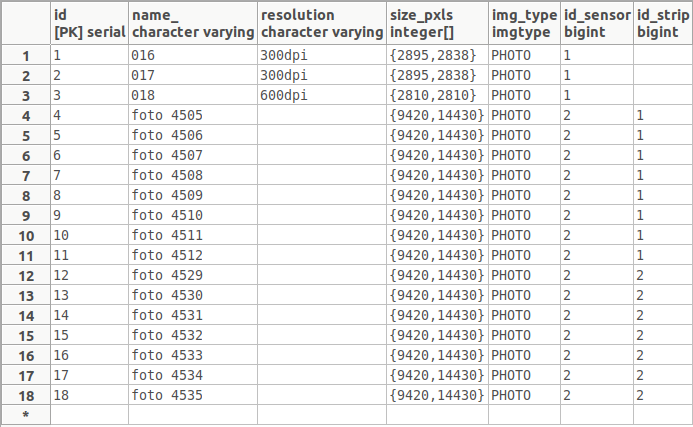
\includegraphics[width=1\hsize]{figuras/img_table.png}
  %\legend{Texto da legenda quando necessário.}
  \source{A autora, 2019.}
\end{figure}

Um banco de dados pode ou não ter a seleção de seus dados armazenados de forma personalizada. Dentre as consultas realizadas, foram elaboradas várias visões. Estas nada mais são que o agrupamento de dados presentes no banco, organizadas de acordo com a programação do usuário. Uma visão pode ser excluída do banco sem que esta signifique que os dados que apresenta sejam perdidos, pois sua exclusão não acarreta na eliminação da tabela original destes dados. Visões também podem ser utilizadas para manter a coerência do banco, auxiliando o DBA a manter um controle do que existe no banco. Um exemplo deste caso é a consulta a seguir:

\begin{lstlisting}
CREATE OR REPLACE VIEW EFOTO.PROJ_LAST_MODIFICATION
AS
SELECT P.NAME_, P.Date_mod
FROM EFOTO.PROJECT P
ORDER BY P.Date_mod DESC;
\end{lstlisting}

A visão deste código apresenta o nome dos projetos existentes no banco, ordenando decrescentemente pela data de modificação. Assim, enquanto não se tem uma forma específica de definir quais projetos estão inativos, esta consulta simples permite ao DBA entender quais projetos não são modificados há mais tempo, o que o auxiliaria na tomada de decisão de manter este projeto no banco ou não. A visão gerada, contendo os dados do banco teste é apresentada na figura \ref{date_mod}.
\begin{figure}[!ht]{10cm}
  \caption{Visão Proj\_last\_modification} \label{date_mod}
  \centering
  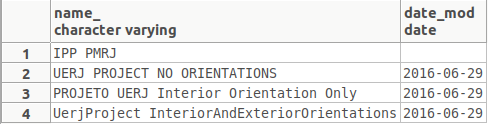
\includegraphics[width=0.8\hsize]{figuras/date_proj.png}
  %\legend{Texto da legenda quando necessário.}
  \source{A autora, 2019.}
\end{figure}
Como visto, nesta visão existe um projeto com o campo de interesse nulo, o que poderia iniciar uma investigação sobre o projeto em questão pelo DBA.

Tratando de consultas à dados fotogramétricos, uma das perguntas feitas foi: \textit{``Quais imagens pertencem à quais projetos?''}, a figura \ref{img_proj}  apresenta 23 tuplas da visão resultante desta pergunta.
\begin{figure}[!ht]{10cm}
  \caption{Visão Img\_proj} \label{img_proj}
  \centering
  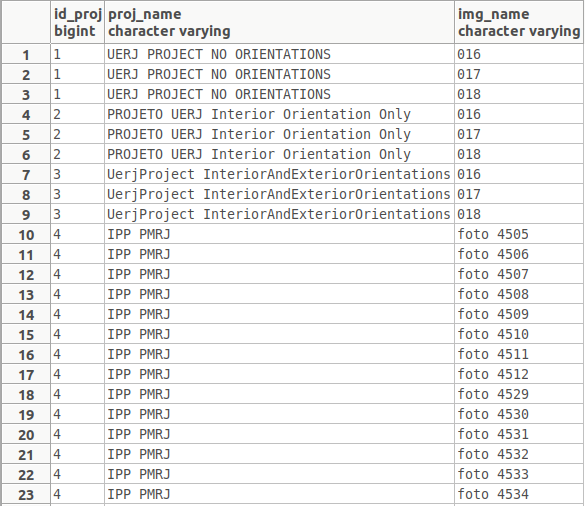
\includegraphics[width=1\hsize]{figuras/img_proj.png}
  %\legend{Texto da legenda quando necessário.}
  \source{A autora, 2019.}
\end{figure}

Como comentado anteriormente ao longo deste trabalho o banco deve ser capaz de armazenar e responder questões sobre dados alfanuméricos e geoespaciais. Assim, perguntas como \textit{``Quais são as coordenadas dos pontos de cada projeto?''}, que pode ser feita também como \textit{``Quais são as coordenadas dos pontos de dado projeto?''} devem ser respondidas. A primeira pode ser respondida numa consulta que, por sua vez, poderia ser uma visão. A segunda pode ser programada como uma função. 

A função \textit{projectpointscoord()}, foi feita para responder justamente esta segunda pergunta. Ao fazer um `select' com esta função, o resultado para o projeto informado pelo usuário, que no caso foi o projeto 4, é apresentado na figura \ref{fun1}. Neste caso o usuário deve somente ter um conhecimento dos índices dos projetos armazenados.

\begin{figure}[!ht]{10cm}
  \caption{Função projectpointscoord} \label{fun1}
  \centering
  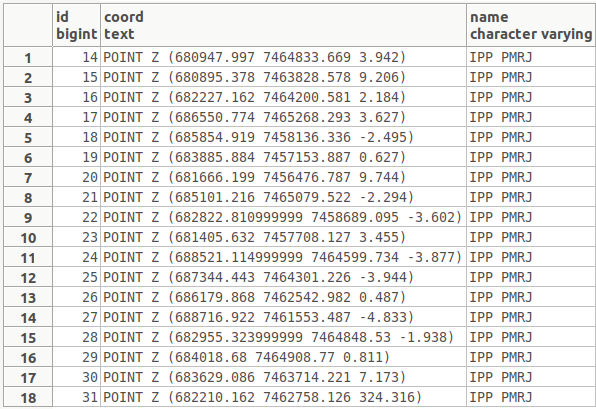
\includegraphics[width=1\hsize]{figuras/fun_ppr.png}
  %\legend{Texto da legenda quando necessário.}
  \source{A autora, 2019.}
\end{figure}

Dessa mesma forma foi criada uma função que responde à consulta: \textit{``Que pontos se encontram dentro de um polígono?''}. Sendo que este polígono poderia ser as delimitações de um ``bounding box'', a projeção de uma foto no terreno ou simplesmente uma área de interesse. O código apresentado a seguir, define a função, \textit{Searchpointsfromgeometry()}, que é capaz de responder esta pergunta.Neste caso os valores de entrada devem estar em WKT, respeitando a sintaxe de um polígono em sql.

\begin{lstlisting}
CREATE OR REPLACE FUNCTION EFOTO.SEARCHPOINTSFROMGEOMETRY(WKT TEXT)
RETURNS TABLE (ID BIGINT, POINT TEXT) AS
$$
SELECT P.ID, ST_AsText(ST_Transform(CAST(P.geom As geometry),32723))
FROM EFOTO.POINT P
WHERE ST_CONTAINS (ST_Transform(ST_GeomFromText(WKT,32723),4326),CAST(P.geom As geometry));
$$ LANGUAGE 'sql';
\end{lstlisting}

Funções, assim como visões, podem ser usadas como ferramentas que testam o banco. Por outro lado ambos os mecanismos podem também facilitar o acesso ao dado pelo usuário comum. A função \textit{Imagekind()} responde ao usuário sobre quais as imagens são de origem digital ou analógica, dependendo somente do usuário informar em qual tipo está interessado. Já a função \textit{EscaleFromImage()} fornece que projetos correspondem ao denominador da escala informada. Neste ponto, para esta última, o usuário deve saber quais valores de escalas estão armazenadas no banco, o que por algumas vezes pode tornar a própria função indesejável, pois antes de executá-la deve ser realizado uma consulta simples que informe quais escalas estão armazenadas no banco de dados. Uma solução para isto é que a função então considere não o denominador de uma escala, mas sim o domínio de denominadores, desde a maior até a menor escala, aumentando, assim, o alcance dessa função.

Com a visão \textit{Image\_file\_found} e sua oposta \textit{Image\_file\_not\_found} é possível saber quais imagens possuem, ou não, arquivos raster armazenados no banco. Isso permite um controle não só do acervo físico do LFSR, mas também auxilia no planejamento das ações tomadas para a aquisição destes arquivos. Estas visões em particular suportam a ideia de que contanto que certos dados dessas imagens sejam conhecidos, como seu local de armazenamento físico, o responsável pelo LFSR será capaz de identificar e realizar um pedido de aquisição para esta foto em caso de imagens de origem analógica, ou arquivo digital em caso de imagens provenientes de imagens digitais.

Um dos questionamentos levantado seria capacidade do banco de responder se: \textit{``O projeto teve sua fase de inicialização finalizada?''}, ou seja, ele está pronto para começar sua geração de produtos? O que de fato define se o projeto já terminou sua fase de inicialização, é a presença dos valores de coeficientes de OI e OE. As visões \textit{Oi\_available} e \textit{Oe\_available} conectam e retornam os valores de cada parâmetro das orientações interior e exterior, às suas respectivas imagens e projetos. As figuras \ref{oi_v} e \ref{oe_v} retornam as visões com os dados até então, carregados no banco de testes.

\begin{figure}[!ht]{13cm}
  \caption{Visão Oi\_available} \label{oi_v}
  \centering
  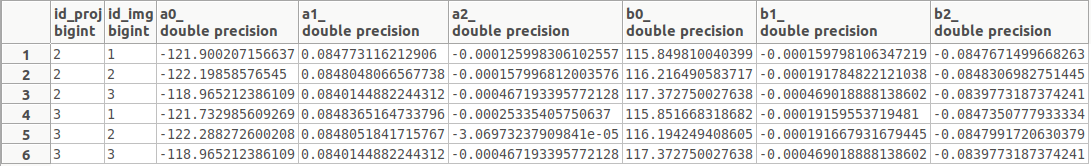
\includegraphics[width=1.1\textwidth, height=0.2\hsize]{figuras/oi.png}
  %\legend{Texto da legenda quando necessário.}
  \source{A autora, 2019.}
\end{figure}
\begin{figure}[!ht]{13cm}
  \caption{Visão Oe\_available} \label{oe_v}
  \centering
  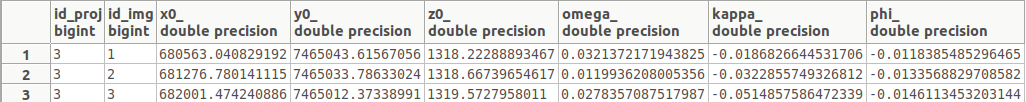
\includegraphics[width=1.1\textwidth, height=0.15\hsize]{figuras/oe.png}
  %\legend{Texto da legenda quando necessário.}
  \source{A autora, 2019.}
\end{figure}

Estas visões por si só, não deixam claro uma resposta para a pergunta em tela. Porém ambas viabilizam a criação de uma nova visão que responda justamente este questionamento. Devido à falta de tempo, a programação e implementação desta visão é prevista em um expansão para o banco de dados. 

Até o momento todas as funções e visões apresentadas foram realizadas separadamente. O código exposto no anexo \ref{script2} comprova que isto não é uma necessidade. Além disto uma pode utilizar da outra para exercer melhor suas finalidades, como é o caso desse código, pois o mesmo expõe os valores dos coeficientes dos parâmetros de OI e OE discutidos acima de uma segunda forma. 

Durante a fase de teste, nem todo o resultado encontrado foi o esperado. Em dado momento, foi levantada a pergunta \textit{``Quantos pontos determinados por Levantamento Topográfico estão armazenados?''}. A resposta dada pelo banco não condizia com a realidade. Neste caso foi investigado qual era a origem deste problema, o que levou à descoberta de um erro no modelo.
Como visto no capítulo \ref{met} existe uma generalização chamada \textit{Survey}, que se especializa nas classes \textit{Ground\_Survey} e \textit{Flight}. Até o momento deste teste, \textit{Collection\_point} realizava uma ligação simples de 1 (um) para 1 (um) com a classe Survey. Isto porém estava errado, pois esta ligação implicava que os pontos de coleções diferentes se confundissem, e o banco, em consequência, duplicava estas coleções sem distinguir de qual levantamento se originavam. A figura \ref{pgs_errado} ilustra a situação ora em questão.

\begin{figure}[!ht]{10cm}
  \caption{Visão Count\_points\_of\_ground\_survey com resultados errados} \label{pgs_errado}
  \centering
  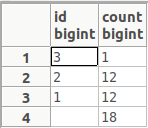
\includegraphics[width=0.3\hsize]{figuras/pgs_errado.png}
  %\legend{Texto da legenda quando necessário.}
  \source{A autora, 2019.}
\end{figure}

Esta ligação então foi refeita ligando as classes \textit{Collection\_point} e \textit{Ground\_Survey}, o que resultou em pequenos ajustes ao longo do modelo. A mesma consulta passou a apresentar os dados de forma correta, como visto na figura \ref{pgs_correto}.

\begin{figure}[!ht]{10cm}
  \caption{Visão Count\_points\_of\_ground\_survey} \label{pgs_correto}
  \centering
  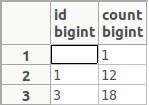
\includegraphics[width=0.3\hsize]{figuras/pgs_correto.png}
  %\legend{Texto da legenda quando necessário.}
  \source{A autora, 2019.}
\end{figure}

Ambas as visões foram geradas graças à consulta abaixo, que define como atributos o índices numéricos de cada \textit{Ground\_Survey} e sua quantidade de pontos, respectivamente.

\begin{lstlisting}

    SELECT GS.ID, COUNT(P.ID)
    FROM EFOTO.POINT P
    LEFT JOIN EFOTO.COLLECTION_POINT CP
    ON P.ID_COLL = CP.ID
    LEFT JOIN EFOTO.GROUND_SURVEY GS
    ON CP.ID_GROUND_SURVEY = GS.ID
    GROUP BY GS.ID ORDER BY COUNT (P.ID);

\end{lstlisting}
Este não foi o único erro descoberto ao longo dos testes, porém todos os problemas encontrados foram resolvidos. Melhorias previstas também foram identificadas, que devido à limitação do tempo, serão deixadas como possíveis expansões para o banco em trabalhos futuros.

Por outro lado, nem todos os contratempos geraram mudanças no modelo. A visualização das imagens armazenadas neste banco de dados piloto não foi feita pelo uso da PgAdmin3. Pois esta interface não têm capacidade de abrir a tabela na qual este arquivo se encontra e nem é idealizada para exibição de imagens. Desta forma foram implementadas duas soluções: a primeira é a presença de um caminho para o local onde o arquivo digital está armazenado, mostrando assim que ele existe no servidor mesmo na hipótese do mesmo não se encontrar fisicamente no banco. A segunda solução foi a visualização dos dados armazenados por meio de outros programas. O script \footnote{Fornecido pelo Professor Irving Badolato, este script é utilizado em suas aulas da disciplina Banco de Dados para ilustrar a recuperação de dados mantidos num servidor PostgreSQl com a extensão Postgis} presente no anexo \ref{script3}, é uma solução que usa o interpretador python para executar um programa descrito desta linguagem e conecta no banco para exibir a imagem armazenada. Para tal, o mesmo faz uso das bibliotecas GDAL, que implementa uma camada de abstração para a manipulação de arquivo de dados geográficos, e o Matplotlib que permite a apresentação de gráficos através de uma janela no Sistema Operacional. Isso prova que podemos expôr o dado em aplicações desenvolvidas no futuro pela equipe do LFSR. Porém, pensando em usuários que não estão familiarizados com a programação, outro meio de visualização dessas imagens foi identificada pela conexão direta com o banco de dados por um software de SIG.

A solução proposta com SIG neste caso é a conexão ao banco pelo QGIS. Neste caso usuário precisa somente se conectar em uma máquina que tenha o acesso ao banco e realizar o acesso pelo software. Feita a conexão o banco as imagens são visualizáveis pelo software QGIS. Nada impede que o usuário procure outros meios de visualização do que os propostos anteriormente. Porém ambos servem para provar que a imagem está acessível pelo banco de dados proposto.

Todos os códigos geradores das funções e visões não referenciados se encontram no apêndice \ref{con}. Ao responder estas e outras perguntas (que tem seus códigos de geração de consulta presentes no apêndice \ref{con}) realizadas pelo responsável de disciplina de fotogrametria do LFSR, o banco pode ser considerado validado.

Devido à complexidade de um processo fotogramétrico e de seus dados, certas limitações se fizeram necessárias para que a realização deste trabalho pudesse cumprir seu prazo estabelecido. Este fato, juntamente com as potencialidades descobertas ao longo do processo, permitiu a previsão de extensões ao modelo elaborado. A modelagem da etapa de produção de um processo fotogramétrico e sua adaptação ao modelo criado por este projeto é um exemplo de expansão prevista. Melhorias que englobem não somente um processo fotogramétrico no nível aéreo, mas também no nível orbital são esperadas e, em alguns casos, sugeridas ao longo do modelo, como discutido neste volume. A criação de uma interface para o banco de dados, vindo a ser este implementado no LFSR, que seja mais amigável ao usuário é também uma possibilidade prevista como extensão e, portanto pode ser desenvolvida em projetos futuros. Por fim, o modelo estabelecido pode ser ampliado para realizar uma integração com a INDE e para possibilitar a execução da restituição estereofotogramétrica diretamente no padrão EDGV. Julga-se que essas atividades sejam passíveis de serem implementadas futuramente no Laboratório.

Vale lembrar que de todos os testes realizados, não houve a realização de nenhum teste de estresse e, que todos os testes e desenvolvimentos explicitados até o presente momento, foram feitos e desenvolvidos para a parte lógica do processo. Desta forma, fica de responsabilidade do LFSR a tomada de decisão de qual espaço físico e como o mesmo será utilizado para a implementação do banco gerado por este trabalho.


